\documentclass[11pt,a4paper,twocolumn]{jsarticle}
%
\usepackage{amsmath,amssymb}
\usepackage{bm}
% 画像がない場合でもコンパイルを通したい場合は、下の行を \usepackage[demo]{graphicx} に変えてください
\usepackage{graphicx}
\usepackage{ascmac}
\usepackage[dvipdfmx]{hyperref}
\usepackage{pxjahyper}

\hypersetup{%
 setpagesize=false,%
 bookmarks=true,%
 bookmarksdepth=tocdepth,%
 bookmarksnumbered=true,%
 colorlinks=true,%
 pdftitle={わかる電子回路 中間レポート},%
 pdfsubject={},%
 pdfauthor={若林 健悟},%
 pdfkeywords={}}
%
\setlength{\textwidth}{\fullwidth}
\setlength{\textheight}{40\baselineskip}
\addtolength{\textheight}{\topskip}
\setlength{\voffset}{-0.2in}
\setlength{\topmargin}{0pt}
\setlength{\headheight}{0pt}
\setlength{\headsep}{0pt}
%
\newcommand{\divergence}{\mathrm{div}\,}
\newcommand{\grad}{\mathrm{grad}\,}
\newcommand{\rot}{\mathrm{rot}\,}
%
\title{わかる電子回路 中間レポート}
\author{氏名：若林 健悟}
\date{学籍番号：J4-251098}

\begin{document}
\maketitle

\section{トランジスタによる論理回路 1}
回路の各部分の電位差、電流を図示すると次のようになる。
\begin{figure}[htbp]
\centering
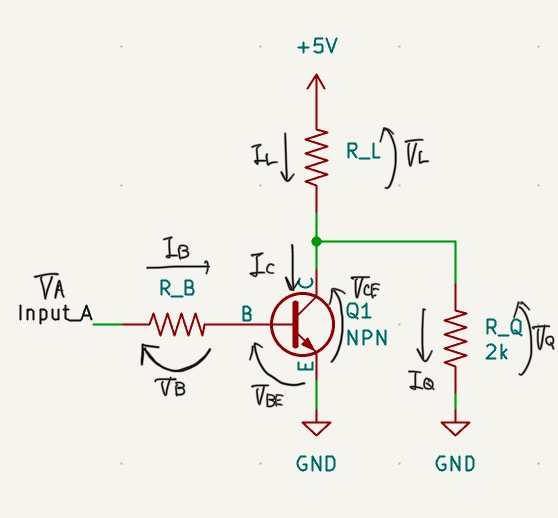
\includegraphics[width=1.0\linewidth]{./image/inverter.jpg}
\caption{電位差と電流の定義}
\end{figure}

従って、回路方程式は、
\begin{align}
V_B+V_{BE}&=V_A \label{eq:1} \\
V_L+V_Q&=V_{CC} \label{eq:2} \\
V_{CE}&=V_Q \label{eq:3} \\
I_Q+I_C&=I_L \label{eq:4} \\
R_BI_B&=V_B \label{eq:5} \\
R_LI_L&=V_L \label{eq:6} \\
RI_Q&=V_Q \label{eq:7} \\
I_{C}&= \beta I_B \label{eq:8}
\end{align}
となる。今、$V_A$の値にかかわらず、$V_{CC}=5, R=2 \times 10^3, \beta = 100$である。

\subsection{\texorpdfstring{$V_A=0$}{VA=0}のとき}
まず、$V_A=0$のとき、すなわち、トランジスタがオフのときを考える。
(\ref{eq:1})と$V_{BE}=0$より、\[V_B=0\]
(\ref{eq:5})に$V_B$を代入すると、$R_B>0$より、\[I_B=0\]
(\ref{eq:8})に$\beta, I_B$を代入すると、\[I_C=0\]
(\ref{eq:4})に$I_C=0$を代入すると、\[I_L=I_Q(=I)\]
(\ref{eq:2}), (\ref{eq:6}), (\ref{eq:7})に$R, V_{CC}, I_L, I_Q$を代入し、さらに$I$を消去すると、\[(1+\frac{R_L}{2\times10^3})V_Q=5\]
この$V_Q$が$V_Q \ge 3$を満たす必要があるので、
\[\frac{5}{1+\frac{R_L}{2\times10^3}} \ge 3\]
\[\therefore R_L \le 1.33 \times 10^3\]

\subsection{\texorpdfstring{$V_A=5.0$}{VA=5.0}のとき}
次に、$V_A=5.0$のとき、すなわち、トランジスタがオンのときを考える。問題文で与えられた工学的近似を用いると、\[V_{BE}=0.7\]
(\ref{eq:1})に$V_A, V_{BE}$を代入すると、\[V_B=4.3\]
(\ref{eq:5})に$V_B$を代入すると、\[I_B= \frac{4.3}{R_B}\]
(\ref{eq:8})に$\beta, I_B$を代入すると、\[I_C=100 \times \frac{4.3}{R_B} = \frac{430}{R_B}\]
(\ref{eq:2})に$V_{CC}$を代入すると、\[V_L=5.0-V_Q\]
(\ref{eq:6})に$V_L$を代入すると、\[I_L= \frac{5.0-V_Q}{R_L}\]
(\ref{eq:4})に$I_C, I_L$を代入すると、\[I_Q=\frac{5.0-V_Q}{R_L} - \frac{430}{R_B}\]
(\ref{eq:7})に$R, I_Q$を代入すると、\[V_Q=2000\times(\frac{5.0-V_Q}{R_L} - \frac{430}{R_B})\]
\[\therefore V_Q=\frac{2000\times(\frac{5.0}{R_L} - \frac{430}{R_B})}{1+\frac{2000}{R_L}}\]
この$V_Q$が$V_Q \le 1$を満たす必要があるので、
\[\frac{10000}{R_L}-\frac{860000}{R_B} \le 1+\frac{2000}{R_L}\]
\[\therefore R_B \le \frac{860000R_L}{8000-R_L}\]
以上より、求める領域は図2のようになる。境界のグラフは$R_B>0, R_L>0$の領域において、$R_L$に関して単調増加であり、その最大値$R_B^{\mathrm{Max}}$は\[R_B^{\mathrm{Max}}=172 \times 10^3\]となる。

\begin{figure}[htbp]
\centering
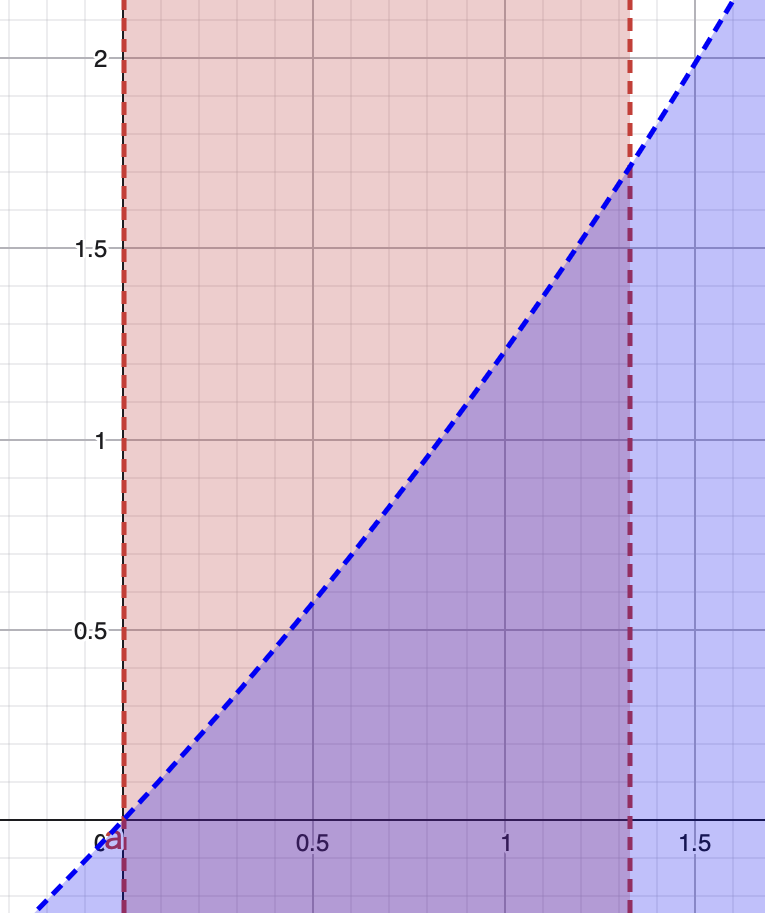
\includegraphics[width=1.0\linewidth]{./image/graph.png}
\caption{求める領域}
\end{figure}

\begin{itembox}[l]{答え}
\[0 \le R_L \le 1.33 \times 10^3\]
\[0 \le R_B \le \frac{860000R_L}{8000-R_L}\]
より、これらの領域に$R_B, R_L$が含まれるように、入手が容易な抵抗で回路を組むとしたら、以下のようにするのが良いと考えられる。
\[R_B=100\,\mathrm{k\Omega}\]
\[R_L=1\,\mathrm{k\Omega}\]
\end{itembox}

\newpage

\section{トランジスタによる論理回路 2}
求める回路は図3のようになると考えられる。

\begin{figure}[htbp]
\centering
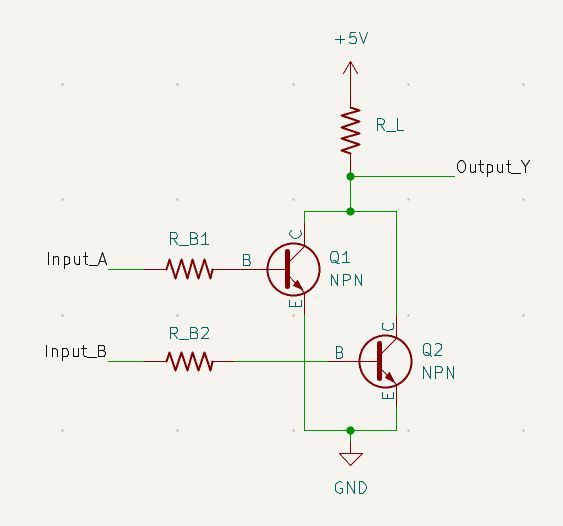
\includegraphics[width=1.0\linewidth]{./image/NOR.png}
\caption{NOR回路}
\end{figure}

\newpage

\section{論理回路を応用した電子回路 1（回路Aの回路図）}
要求される機能は、NAND回路、NOT回路、スイッチング回路を順に接続すれば得られるので、これをトランジスタと抵抗で実現すると図4のようになると考える。

\begin{figure}[htbp]
\centering
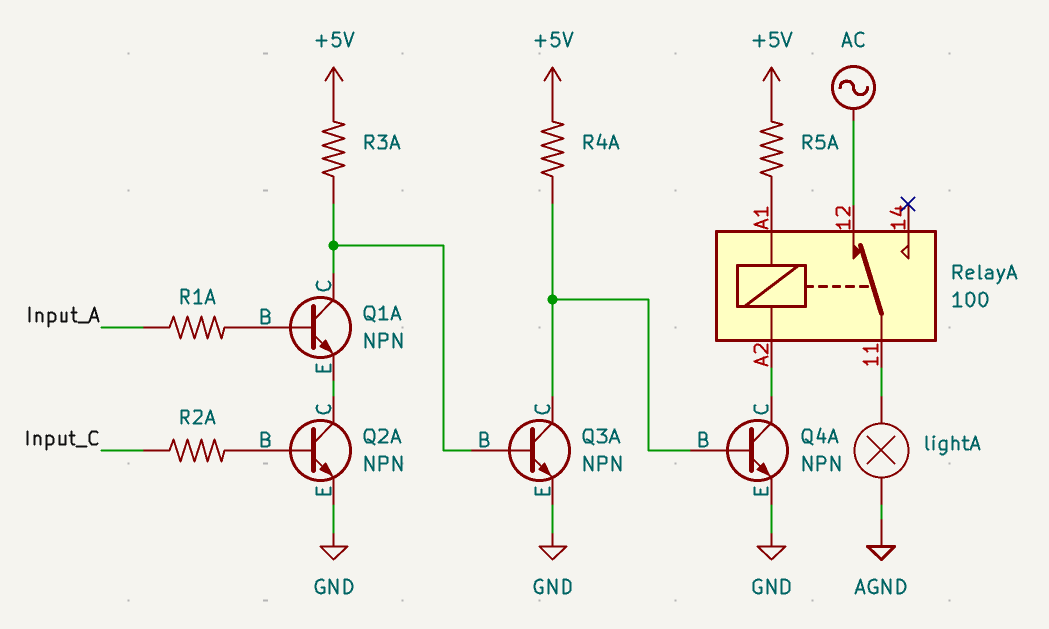
\includegraphics[width=0.8\linewidth]{./image/circuitAa.png}
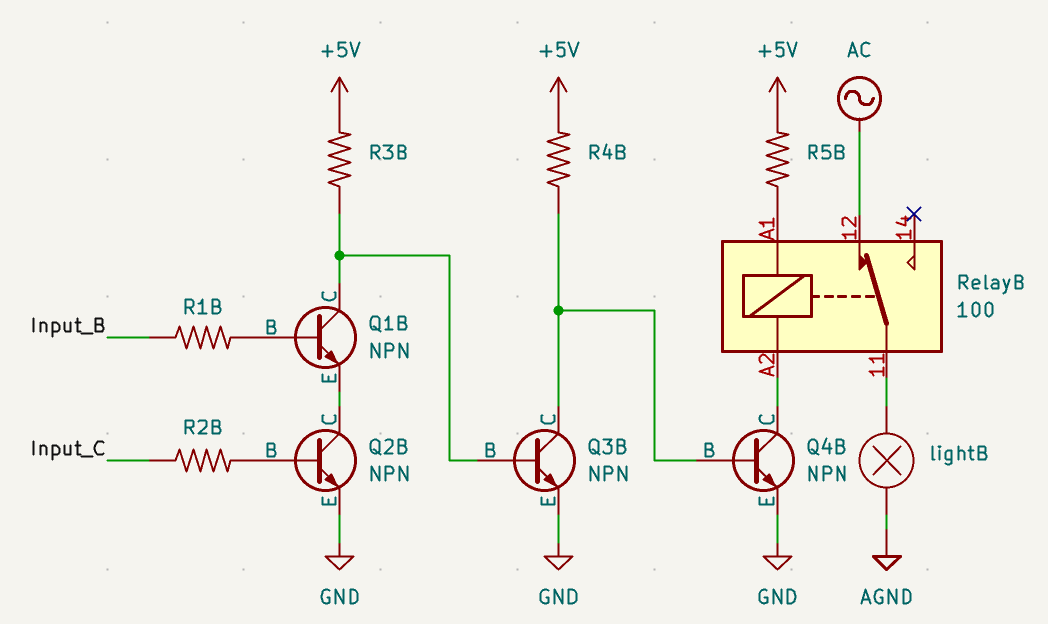
\includegraphics[width=0.8\linewidth]{./image/circuitAb.png}
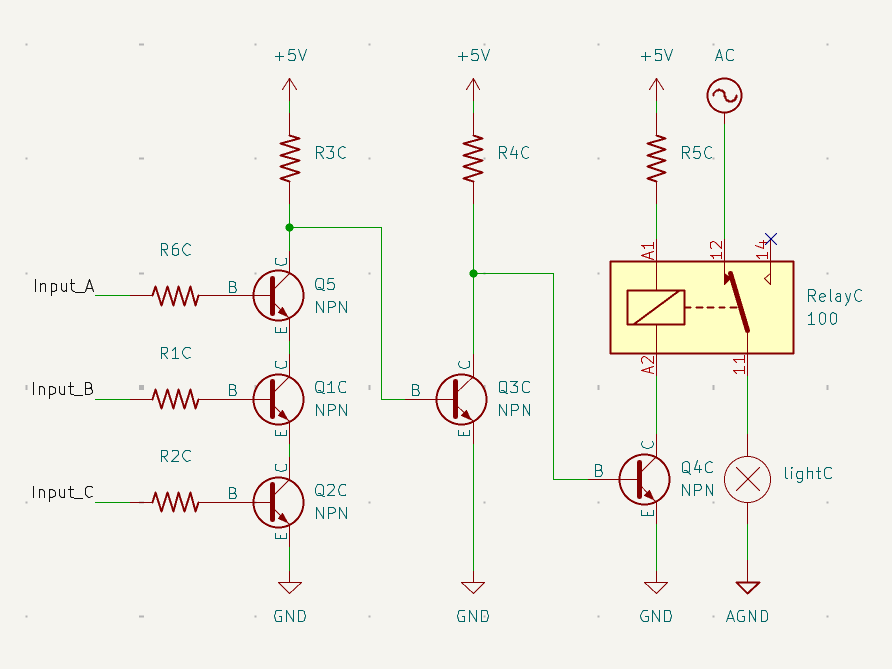
\includegraphics[width=0.8\linewidth]{./image/circuitAc.png}
\caption{回路Aの回路図}
\end{figure}

\newpage

\section{論理回路を応用した電子回路 2（Rの決定）}
回路方程式を解いて各抵抗値を決定する。ここで、リレーの内部抵抗を$100\,\Omega$と仮定した。

\subsection{2入力AND回路の場合}
\subsubsection{Q1,Q2が両方ONになるとき}
トランジスタQ1,Q2が両方ONになるときを考える。この時、Q3はOFF、Q4はONになる。Q1, Q2のコレクタ-エミッタ間に流れる電流を$100I$とおき、キルヒホッフの法則とトランジスタの増幅率の式$I_C=\beta I_B$から回路の各部分にかかる電圧と流れる電流を求めると次のようになる。ここで、$V_{CC}=5, \beta =100, V_{BE}=0.7, V_{CE}=0.2$と近似でき、Q4のコレクタ-エミッタ間に流れる電流が$43\,\mathrm{mA}$となるように設計することを用いた。

\begin{figure}[htbp]
\centering
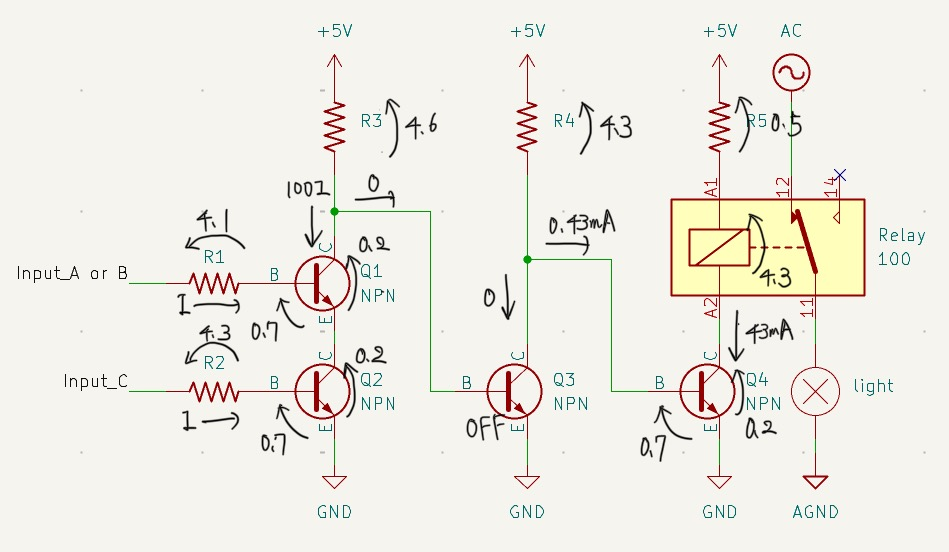
\includegraphics[width=1.0\linewidth]{./image/circuitP1.jpg}
\caption{Q1,Q2が両方ONになるときの電位差と電流}
\end{figure}

ここで、オームの法則を各抵抗に用いると、
\begin{align}
R_1I&=4.1 \label{eq:p1} \\
R_2I&=4.3 \label{eq:p2} \\
100R_3I&=4.6 \label{eq:p3} \\
R_4&=10 \times 10^3 \label{eq:p4} \\
R_5&=11.6 \label{eq:p5}
\end{align}
となる。

\subsubsection{Q1,Q2の少なくとも一方がOFFになるとき}
トランジスタQ1,Q2の少なくとも一方がOFFになるときを考える。この時、Q3はON、Q4はOFFになる。Q3のベース-エミッタ間に流れる電流を$I'$とおき、キルヒホッフの法則とトランジスタの増幅率の式から回路の各部分にかかる電圧と流れる電流を求めると次のようになる。

\begin{figure}[htbp]
\centering
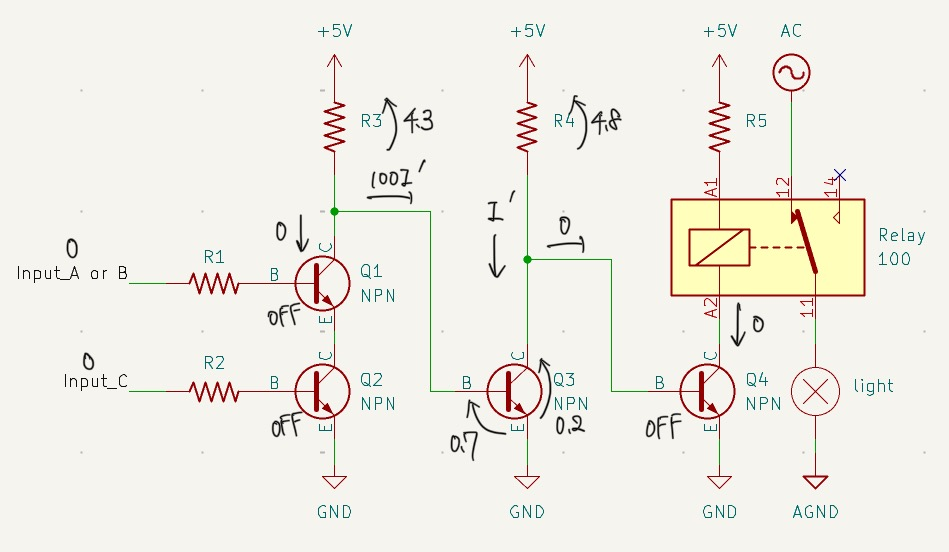
\includegraphics[width=1.0\linewidth]{./image/circuitP2.jpg}
\caption{Q1,Q2の少なくとも一方がOFFになるときの電位差と電流}
\end{figure}

ここで、オームの法則を各抵抗に用いると、
\begin{align}
R_3I'&=4.3 \label{eq:p6} \\
100R_4I'&=4.8 \label{eq:p7}
\end{align}
となる。

これまで立てた方程式を連立して、不明な抵抗値$R_1,R_2,R_3$と電流$I, I'$を求める。
(\ref{eq:p7})に(\ref{eq:p4})の$R_4$を代入すると、\[I'=4.8 \times 10^{-6}\]
(\ref{eq:p6})に$I'$を代入すると、\[R_3=\frac{4.3}{4.8 \times 10^{-6}} \approx 896 \times 10^3\]
(\ref{eq:p3})に$R_3$を代入すると、\[I=\frac{4.6}{100\times 8.96 \times 10^5} \approx 5.13 \times 10^{-8}\]
(\ref{eq:p1}), (\ref{eq:p2})に$I$を代入すると、\[R_1=\frac{4.1}{5.13 \times 10^{-8}} \approx 80\times 10^6\]
\[R_2=\frac{4.3}{5.13 \times 10^{-8}} \approx 84\times 10^6\]

\begin{itembox} [l]{動作限界の抵抗値（理論値）}
\[R_1 \approx 80\,\mathrm{M\Omega}\]
\[R_2 \approx 84\,\mathrm{M\Omega}\]
\[R_3 \approx 896\,\mathrm{k\Omega}\]
\[R_4 = 10\,\mathrm{k\Omega}\]
\[R_5 = 11.6\,\Omega\]
\end{itembox}

\subsection{3入力AND回路の場合}
2入力AND回路との差異は、3つ目の抵抗とトランジスタのみであるから、トランジスタQ1,Q2,Q5の少なくとも一つがOFFのときの回路方程式は2入力AND回路の場合と同じである。
従って、$I'$と$R_3, R_4, R_5$の値は同じである。

次に、トランジスタQ1,Q2,Q5が全てONになるときを考える。この時、Q3はOFF、Q4はONになる。Q1, Q2, Q5のコレクタ-エミッタ間に流れる電流を$100I$とおき、キルヒホッフの法則とトランジスタの増幅率の式から回路の各部分にかかる電圧と流れる電流を求めると次のようになる。

\begin{figure}[htbp]
\centering
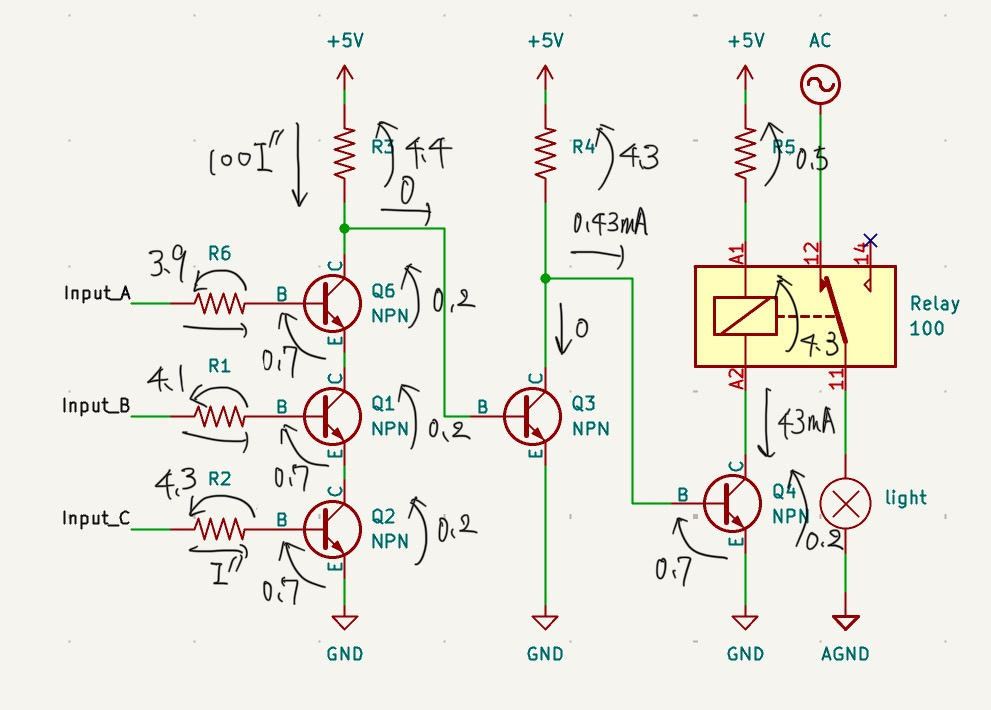
\includegraphics[width=1.0\linewidth]{./image/circuitP3.jpg}
\caption{Q1,Q2,Q5が全てONになるときの電位差と電流}
\end{figure}

ここで、オームの法則を各抵抗に用いると、
\begin{align}
R_1I''&=4.1 \label{eq:p8} \\
R_2I''&=4.3 \label{eq:p9} \\
R_6I''&=3.9 \label{eq:p10} \\
100R_3I''&=4.4 \label{eq:p11}
\end{align}
となる。
これまで立てた方程式を連立して、不明な抵抗値$R_1,R_2, R_6$と電流$I''$を求める。
(\ref{eq:p11})に$R_3$を代入すると、\[I''=4.91 \times 10^{-8}\]
(\ref{eq:p8}), (\ref{eq:p9}), (\ref{eq:p10})に$I''$を代入すると、\[R_1=\frac{4.3}{4.91 \times 10^{-8}} \approx 87.6 \times 10^6\]
\[R_2=\frac{4.1}{4.91 \times 10^{-8}} \approx 83.5 \times 10^6\]
\[R_6=\frac{3.9}{4.91 \times 10^{-8}} \approx 79.4 \times 10^6\]

\begin{itembox} [l]{動作限界の抵抗値（理論値）}
\[R_1 \approx 88\,\mathrm{M\Omega}\]
\[R_2 \approx 84\,\mathrm{M\Omega}\]
\[R_3 \approx 896\,\mathrm{k\Omega}\]
\[R_4 = 10\,\mathrm{k\Omega}\]
\[R_5 = 11.6\,\Omega\]
\[R_6 \approx 79\,\mathrm{M\Omega}\]
\end{itembox}

\subsection{実用回路における抵抗値の決定}
前節までの計算で得られた抵抗値は、問題で与えられた$I_{CE} = \beta I_B$ が厳密に成り立つ場合の理論上の最大抵抗値である。

本回路のトランジスタ$Q_1, Q_2, Q_3, Q_5$はスイッチとして動作させるため、トランジスタを確実にON状態にする必要がある。このとき、ベース電流 $I_B$ を増幅動作時よりも十分に多く流す必要があり、以下の不等式を満たす必要がある。
\[ I_B > \frac{I_{CE}}{\beta} \]
これは、抵抗値 $R$ においては、前節で求めた理論値 $R_{\mathrm{limit}}$ に対して、
\[ R < R_{\mathrm{limit}} \]
となるような値を設定することと等価である。

計算された理論上限値は数$M\Omega$と非常に大きな値であるため、これよりも十分に小さく、かつ入手が容易な抵抗値を選定することで、バラツキや温度変化に対しても安定したスイッチング動作が保証されると考えられる。

そこで、実際の回路における値を以下のように決定する。

\begin{itemize}
    \item $R_1, R_2, R_6$について \\
    理論上限は約 $80\mathrm{M}\Omega$ である。これより十分に小さく、一般的な抵抗の値である $100\mathrm{k}\Omega$ を採用する。
    \[ R_1 = R_2 = R_6 = 100\,\mathrm{k}\Omega \]

    \item $R_3$について \\
    理論上限は$896\mathrm{k}\Omega$ である。同様に、十分小さい値として $10\mathrm{k}\Omega$ を採用する。
    \[ R_3 = 10\,\mathrm{k}\Omega \]

    \item $R_4, R_5$について \\
    $R_4$については、計算結果が$10\mathrm{k}\Omega$であるから、この値を採用する。$R_5$については、計算値 $11.6\,\Omega$ に近い標準的な抵抗値を選定する。したがって、
    \[ R_5 = 10\,\mathrm{k}\Omega \]
    \[ R_5 = 10\,\Omega \]
\end{itemize}

以上より、最終的な実装回路の定数を決定した。

\begin{itembox}[l]{最終決定した抵抗値}
\[R_1 = R_2 = R_6 = 100\,\mathrm{k}\Omega\]
\[R_3 = R_4 = 10\,\mathrm{k}\Omega\]
\[R_5 = 10\,\Omega\]
\end{itembox}

\newpage

\section{論理回路を応用した電子回路 3（回路Bの回路図）}
回路Bとして、AND回路とスイッチング回路を合わせた図8のような回路が考えられる。
\begin{figure}[htbp]
\centering
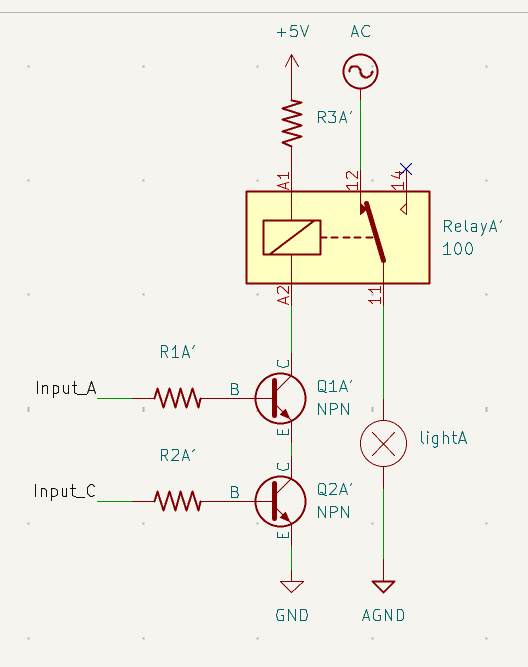
\includegraphics[width=0.8\linewidth]{./image/circuitBa.png}
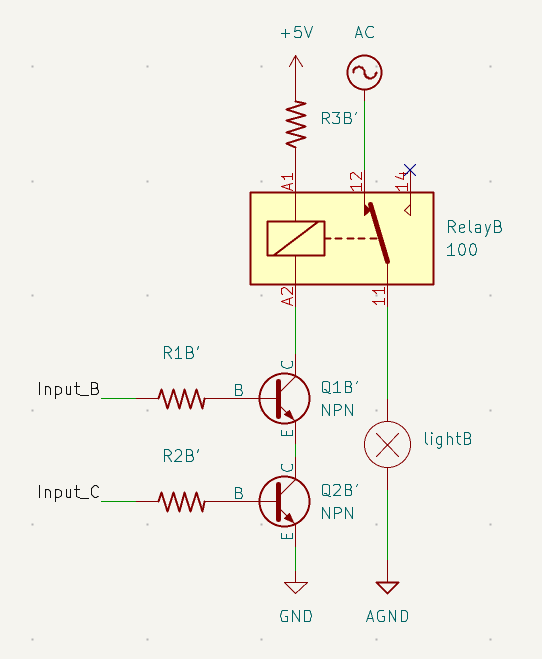
\includegraphics[width=0.8\linewidth]{./image/circuitBb.png}
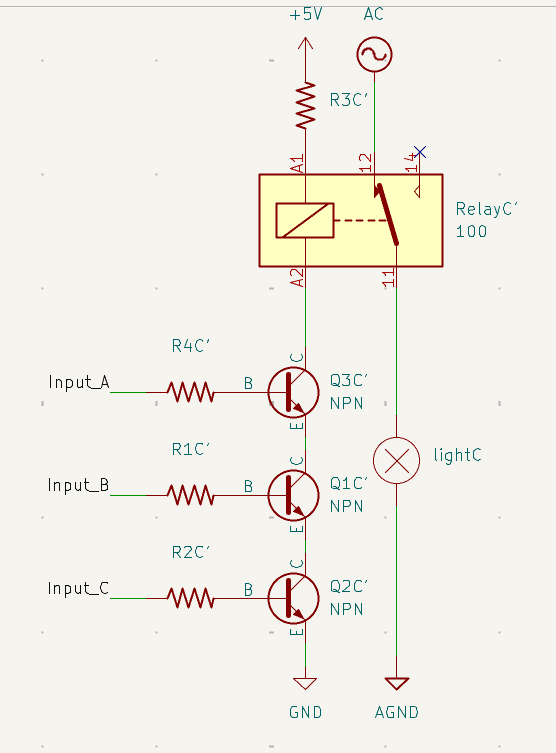
\includegraphics[width=0.8\linewidth]{./image/circuitBc.png}
\caption{回路Bの回路図}
\end{figure}

\section{論理回路を応用した電子回路 4（回路Aと回路Bの得失）}
部品点数、入力に必要な電流、動作の安定性、メンテナンス性といった点で差異が見られる。

\subsection{部品点数}
回路Aはトランジスタを13個も使用しないといけないが、回路Bでは7個で済むため、回路Bの方が優れている。

\subsection{入力に必要な電流}
入力に必要な電流は、回路Aでは問題4で求めたように$I \approx 5.13\times10^{-8}\,\mathrm{A}$であるが、回路Bでは$43\,\mathrm{mA}$のコレクタ電流を得るために、$\beta=100$とするとベース電流は $\frac{43\,\mathrm{mA}}{100}=0.43\,\mathrm{mA} (= 4.3 \times 10^{-4}\,\mathrm{A})$ 必要であり、回路Bの方が約10000倍大きい。従って、入力をマイコンなどで行う際には、回路Aの方が小電流で済むため安全面で優れている。

\subsection{動作の安定性}
回路Aは、論理段数が増えてもリレーを駆動する最終段のトランジスタは常に1個であるため、リレーにはほぼ電源電圧に近い電圧が印加され、安定して動作するが、回路Bはトランジスタを直列に接続するため、段数が増えるごとにコレクタ-エミッタ間飽和電圧の$0.2\,\mathrm{V}$が加算されて電圧降下が生じる。今回の3入力程度であれば問題ないが、入力数が増加した場合、リレーへの印加電圧不足により動作しないリスクが高まる。従って、多入力への動作安定性という点では回路Aが優れている。

\subsection{メンテナンス性}
回路Aは機能ごとにブロックが独立しているため、故障が発生した際に、論理ゲート部分の故障かスイッチング部分の故障かを切り分けてデバックすることが容易である。 対して回路Bではそれらが一体化しているため、リレーが動作しない場合に特定のトランジスタの故障なのか、あるいは前段の入力電圧不足なのかを切り分けることが難しく、メンテナンス性に劣る。

\section{調査課題}
交通渋滞モデルについて調べた。信号や物理的な障害物が存在しない道路区間でも、交通渋滞が起こることは有名である。これを自然渋滞といい、交通流内部の微小な揺らぎが増幅されることで発生する。この現象を、流体力学を交通渋滞に適応したモデルである、KWモデルを用いて考察する。

\subsection{モデルの定義}
まず、道路が一方通行であり、周回や分かれ道を持たないと仮定する。例えば、高速道路のある区間などを思い浮かべて貰えばわかりやすいと思う。この時、ある車両の中心の位置$\boldsymbol{r_i}$は、原点から道路に沿って測った長さ$x_i$を用いて、$\boldsymbol{r_i}=x_i$と表される。
すなわち、原点から道路に沿った1次元座標を考えて運動を議論することができる。

次に、以下の3つの物理量を導入する。
\begin{enumerate}
\item 交通密度 $\rho$: 単位長さあたりの道路区間に存在する車両の台数
\item 交通量 $Q$: 単位時間あたりにある地点 $x_i$ を通過する車両の台数
\item 速度場 $v$: ある区間内の車両の平均的な移動速度
\end{enumerate}

$\rho, Q, v$ は全て $(x, t)$ に依存する関数である。$\rho, Q, v$はそれぞれ、流体力学における流体密度、流量、流速に対応している。したがって、これらの間には、
\[Q=\rho \cdot v\]
の関係が成り立っている。また、$\rho, Q, v$は全て$(x,t)$に依存する関数である。

次にこれらの物理量の間に成り立つ関係式について考える。車両の出入りがない限り、区間内の車両台数は保存される。微小な区間 $dx$ と微小な時間 $dt$ を考えたとき、その区間内の車両数の時間変化率は、区間への流入量と流出量の差に等しい。したがって、以下の偏微分方程式が成り立つ。これは流体力学における連続の式に対応する。
\[\frac{\partial \rho(x,t)}{\partial t} + \frac{\partial Q(x,t)}{\partial x} = 0\]

しかし、$Q=\rho \cdot v$であるから、この偏微分方程式には、未知関数が $\rho$と $v$の2つ含まれており、このままでは解くことができない。したがって、速度 $v$ が密度 $\rho$ の関数であることを仮定してみる。すなわち、
\[v = v(\rho)\]
とする。すると、$Q=\rho \cdot v$より、
\[Q(\rho)=\rho v(\rho)\]
と、$Q$を$\rho$の関数として表すことができる。道路が空いている（$\rho \approx 0$）ときは車両は制限速度などの最高速度 $v_{\mathrm{max}}$ で走行し、混雑して密度が高くなるにつれて速度は低下し、最大の混雑密度 $\rho_{\mathrm{max}}$に達すると速度が $0$ になるという感じで、$v$が$\rho$に伴って変化すると仮定することは、日常的な感覚とも矛盾しない。

この $Q(\rho)$ を元の連続の式に代入すると、$\rho$に関する偏微分方程式が得られる。

\[\frac{\partial \rho(x,t)}{\partial t} + \frac{dQ(\rho)}{d\rho} \frac{\partial \rho(x,t)}{\partial x} = 0\]
この微分方程式を解くことにより、任意の$(x,t)$における$\rho$を求めることができる。

ここで、$c(\rho) = \frac{dQ}{d\rho}$ は、交通量の微小な変化が伝わる速度を表す。これを特性速度という。これを用いると、渋滞が起こっている区間と渋滞が起こっていない区間の境界面の移動速度、すなわち、渋滞の最後尾の伝播速度$U$を算出することができる。
\[U=\frac{Q(\rho_{\mathrm{jam}})-Q(\rho_{\mathrm{free}})}{\rho_{\mathrm{jam}}-\rho_{\mathrm{free}}}\]

\subsection{シミュレーションとその考察}
Pythonで実際に車両密度$\rho(x,t)$がどう変化し、渋滞と自由流の境界がどのように移動するのかをシミュレーションしてみた。先ほどの$\rho$に関する偏微分方程式をゴドノフ法を使って解き、車両密度$\rho(x,t)$の変化をグラフで表示するようにした。また、実際の車両の走行の様子も可視化してわかりやすいようにした。\\
ソースコードはこのGitHubに置いてあるので、興味があれば見てください。\\
\url{https://github.com/Gonke0606/wakaden25.git}\\

シミュレーションの設定は以下の通り。
\begin{enumerate}
\item 円形で分かれ道のない長さ$1000[\mathrm{m}]$の道路を考える。車両の位置は始点から円に沿って測った距離$x (0\le x\le 1000)$で指定する。
\item 車両は渋滞がなければ法定速度$v_{\mathrm{max}}$で走行し、追い越ししない。
\item $600\le x\le 800$の区間は速度が他よりも小さいボトルネック区間となっている。上り坂やトンネルなどをイメージしてもらえるとわかりやすいと思う。
\item $\rho$と$v(\rho)$の初期条件は次の通り。
\[\rho_{\mathrm{init}} = 0.025[\text{台}/\mathrm{m}]\]
\[v_{\mathrm{init}}(\rho) = 20.0[\mathrm{m/s}]\]
\end{enumerate}

この設定でシミュレーションを行うと次のようになった。
\begin{figure}[htbp]
\centering
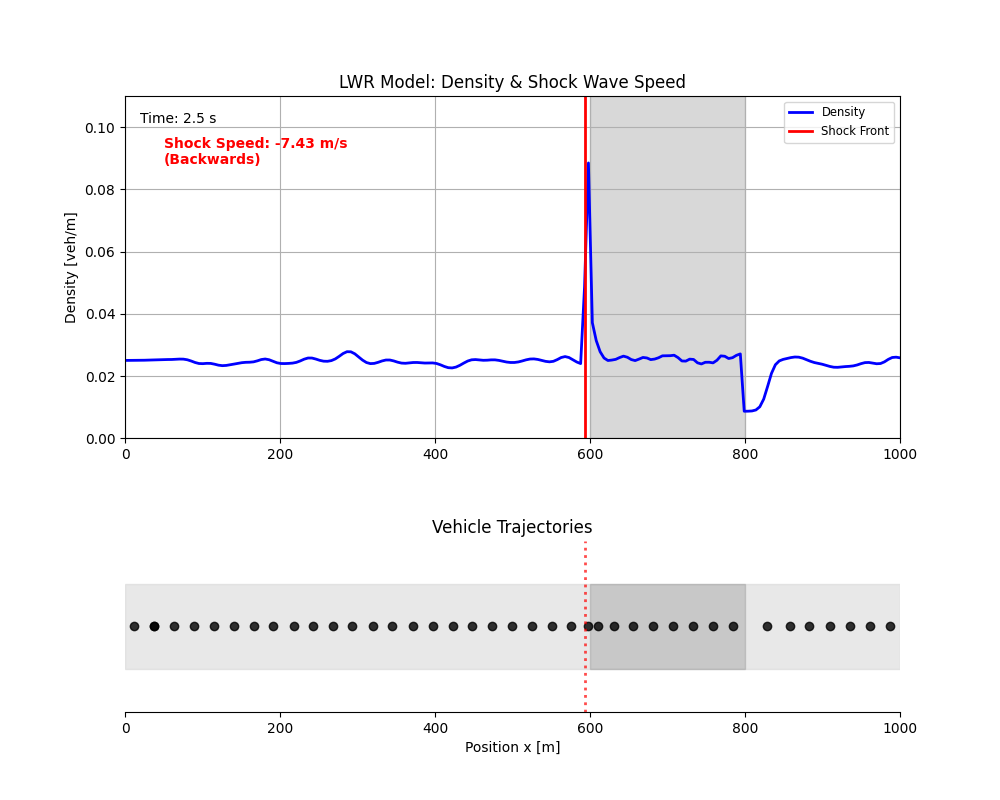
\includegraphics[width=0.9\linewidth]{./image/simulation1.png}
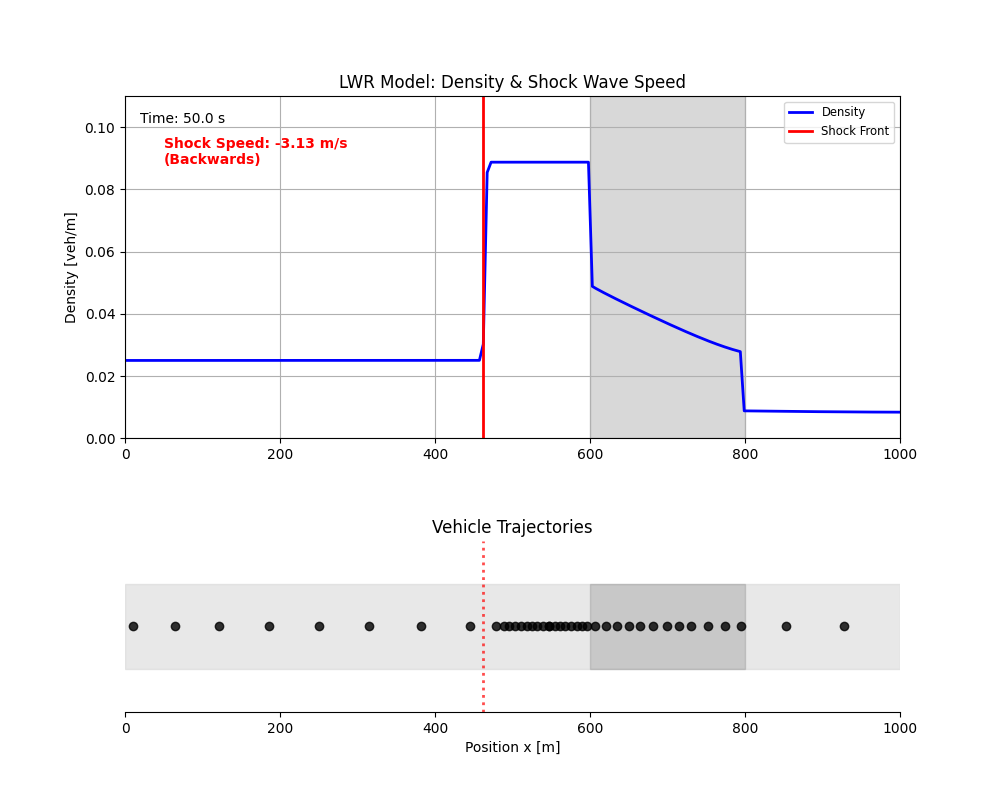
\includegraphics[width=0.9\linewidth]{./image/simulation2.png}
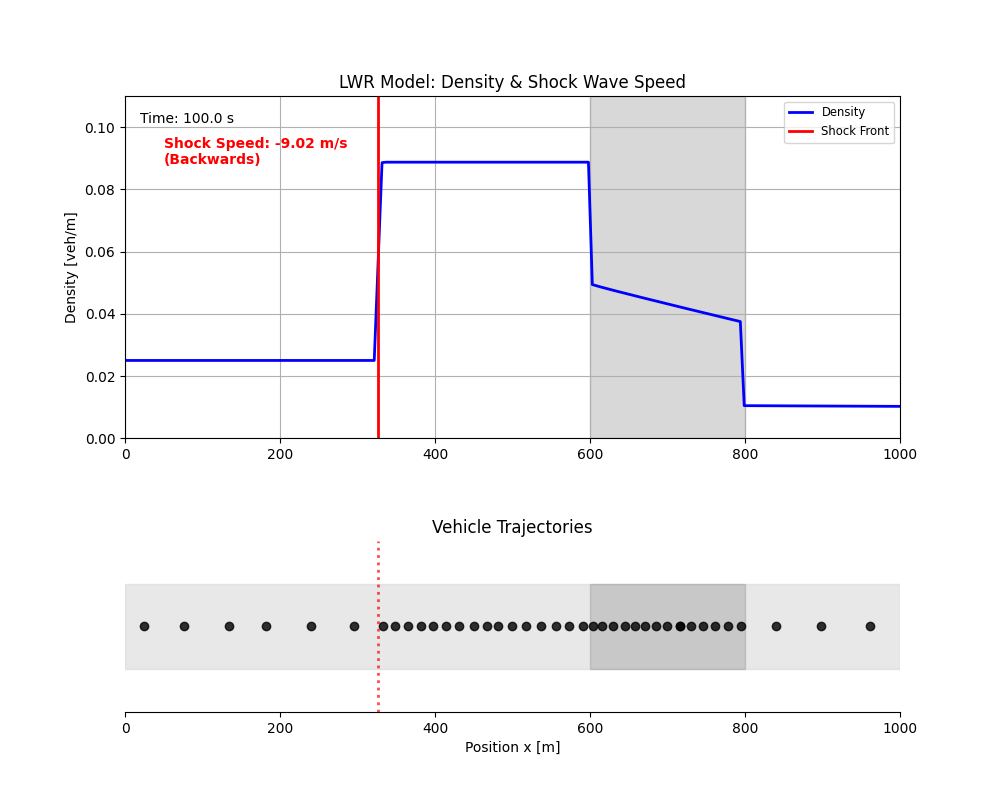
\includegraphics[width=0.9\linewidth]{./image/simulation3.png}
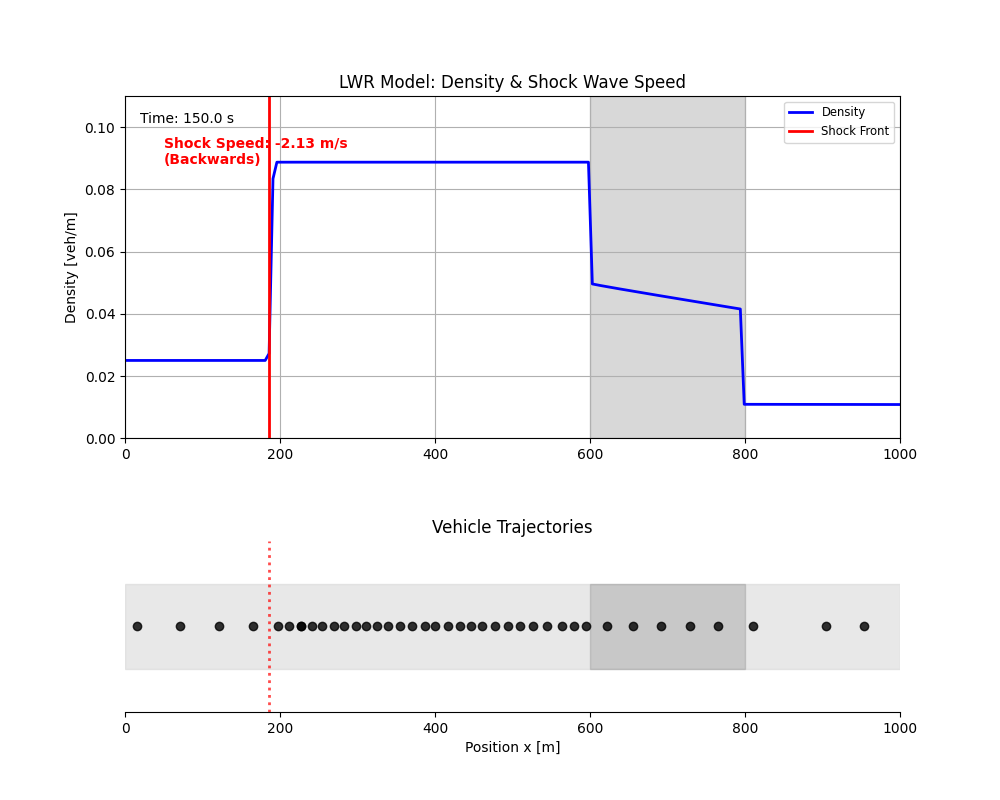
\includegraphics[width=0.9\linewidth]{./image/simulation4.png}
\caption{シミュレーションの結果}
\end{figure}

この結果から、なんらかの原因で一部の車両の速度が遅くなると、確かに渋滞が自然発生することと、渋滞の最後尾は車両の進行方向とは逆方向に伝播することがわかった。後者は、$\rho_{\mathrm{jam}}>\rho_{\mathrm{free}}$であるから、$\rho_{\mathrm{jam}}-\rho_{\mathrm{free}}>0$となるが、$Q(\rho_{\mathrm{jam}})<Q(\rho_{\mathrm{free}})$であるため、$Q(\rho_{\mathrm{jam}})-Q(\rho_{\mathrm{free}})<0$となり、$U<0$となるからだと考えられる。

このように、KWモデルを使って自然渋滞の発生をシミュレーションすることができた。しかし、KWモデルは粘性項を含まないため、渋滞の最後尾が不連続な面として維持され続ける。一方、現実の交通流では、ドライバーの反応遅れや加減速の滑らかさが存在するため、境界面はもう少し連続的な遷移領域を持つと予想される。より現実に近いシミュレーションを行うには、反応遅れを考慮した微視的モデルや、粘性項を加えたモデルへの拡張をする必要があると考えられる。

\section{アンケートと最終課題について}
部品の挙動について今まで感覚的にしかわかっていなかったのが、授業を通して定量的に扱えるようになり、世界が広がった気がする。また、座学だけでなく実際に部品を動かして計測を行うことで、実感を伴って理解できるのがいいと思った。僕はフランス語選択なので、時折挟まれるフランス語の話題は、普段の学習の刺激にもなり楽しく聞かせてもらっている。改善点として思っているのは、授業が月曜1限で起きるのが辛いところと、演習の時間がないため内容が身についているか確認しづらい点である。これからもご指導よろしくお願いします。

最終課題だが、磁界共鳴型のワイヤレス給電器を製作してみたいと考えている。ワイヤレス給電の方式は様々なものがあるが、現在主流なのは電磁誘導を用いた方式だ。しかし、電磁誘導方式は簡単に作れる反面、位置ずれに弱く伝送距離が弱いという欠点がある。一方、磁界共鳴方式とは、受電側にコンデンサを加えて送電側との周波数を合わせることによって共鳴を起こし、磁場から得られるエネルギーを最大化することによって伝送距離を伸ばす手法である。この方式は電磁誘導の回路にコンデンサを追加するだけで実現できるので今回の開発期間でもなんとか形にできるのではないかと考えた。ここで障壁となるのは、共振周波数をピッタリ一致させないと共振が起きず電磁誘導の場合と変わらない伝送距離になってしまう点である。

現在の進捗については、とりあえず電磁誘導方式で電力を送れるところまではできた。回路の構成としては、送電側はZVS発振回路を用いて正弦波を作り、それをリッツ線で自作したコイルに送る構成になっている。一方受電側は単にコイルで受け取った電流を整流してLEDを光らせる構成になっている。

\begin{figure}[htbp]
\centering
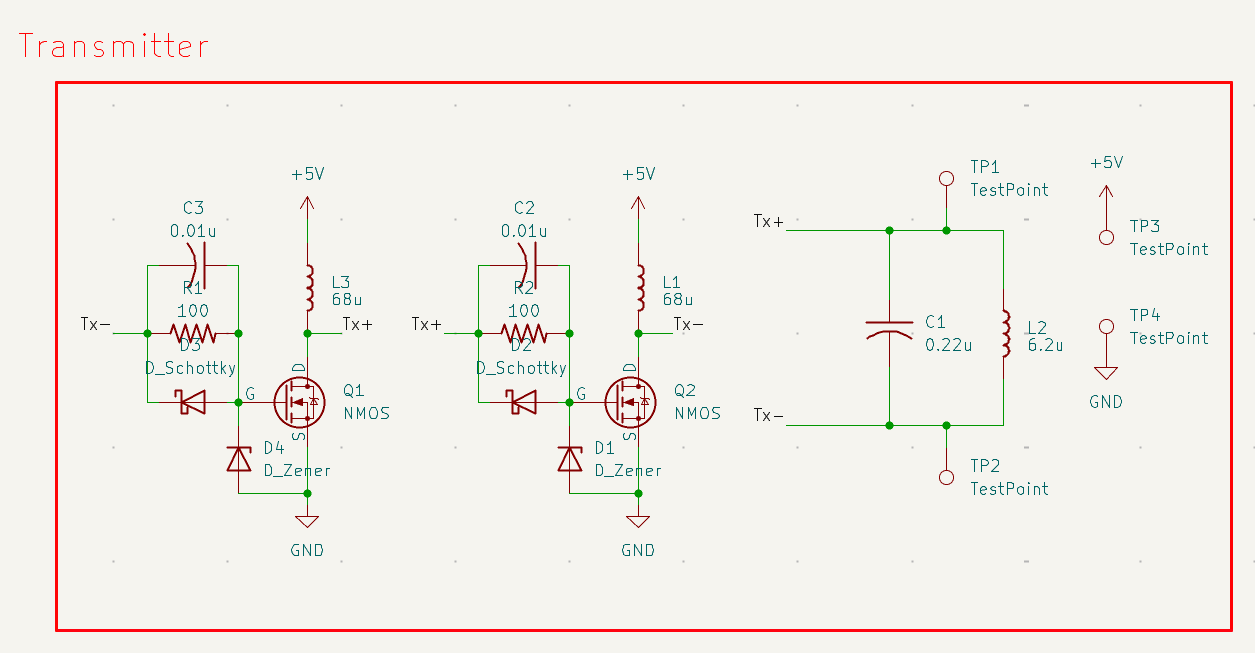
\includegraphics[width=1.0\linewidth]{./image/wireless1.png}
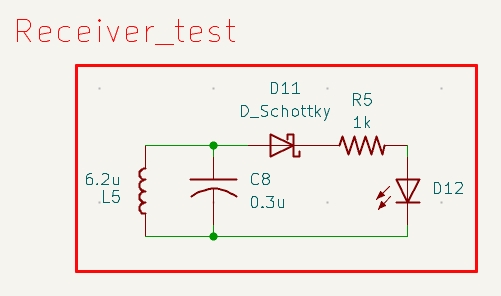
\includegraphics[width=0.8\linewidth]{./image/wireless2.png}
\caption{送信側と受信側の回路図（暫定）。}
\end{figure}

\begin{figure}[htbp]
\centering
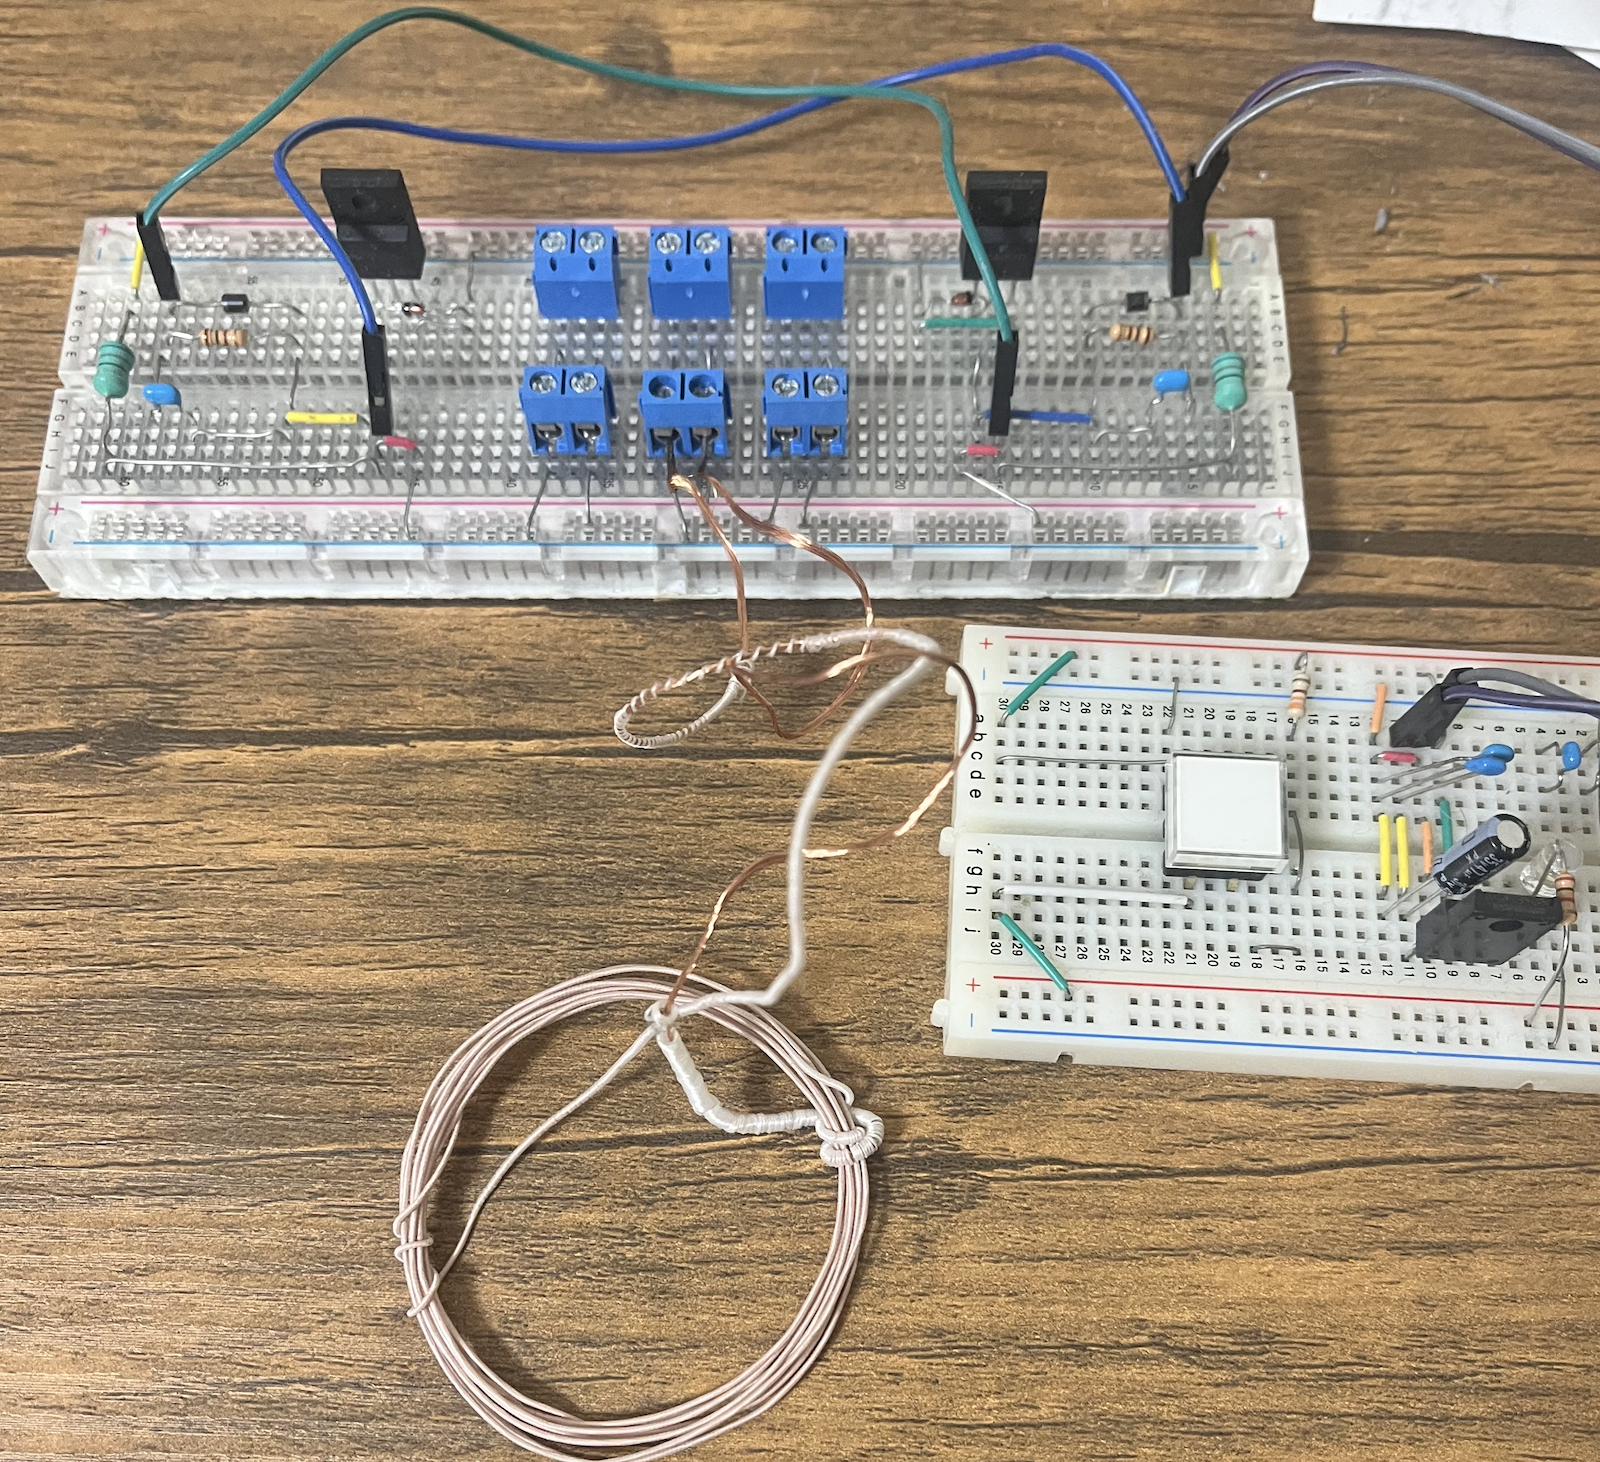
\includegraphics[width=0.8\linewidth]{./image/wireless3.png}
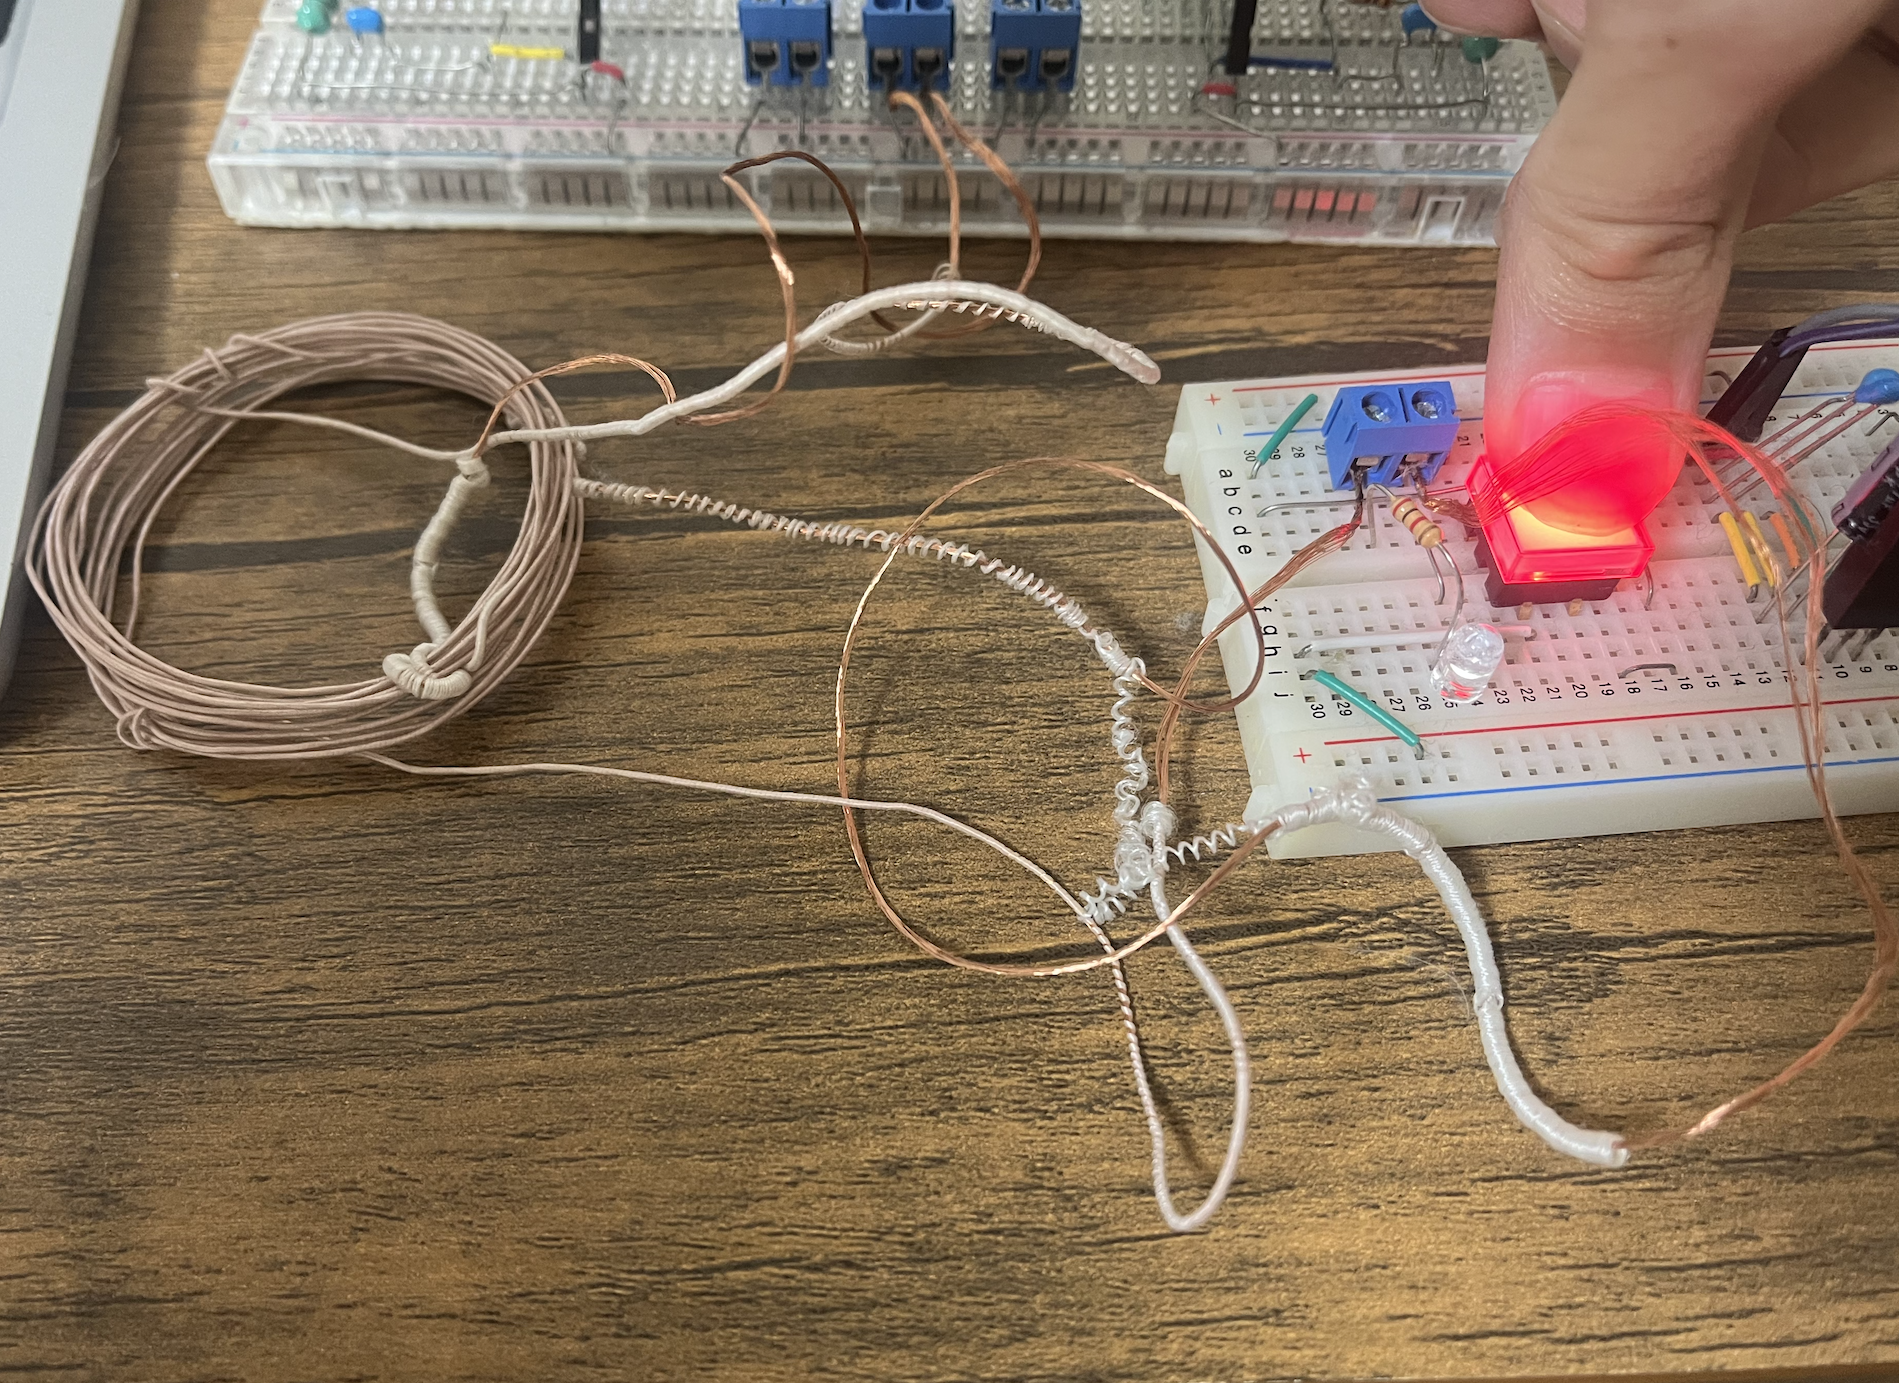
\includegraphics[width=0.8\linewidth]{./image/wireless4.png}
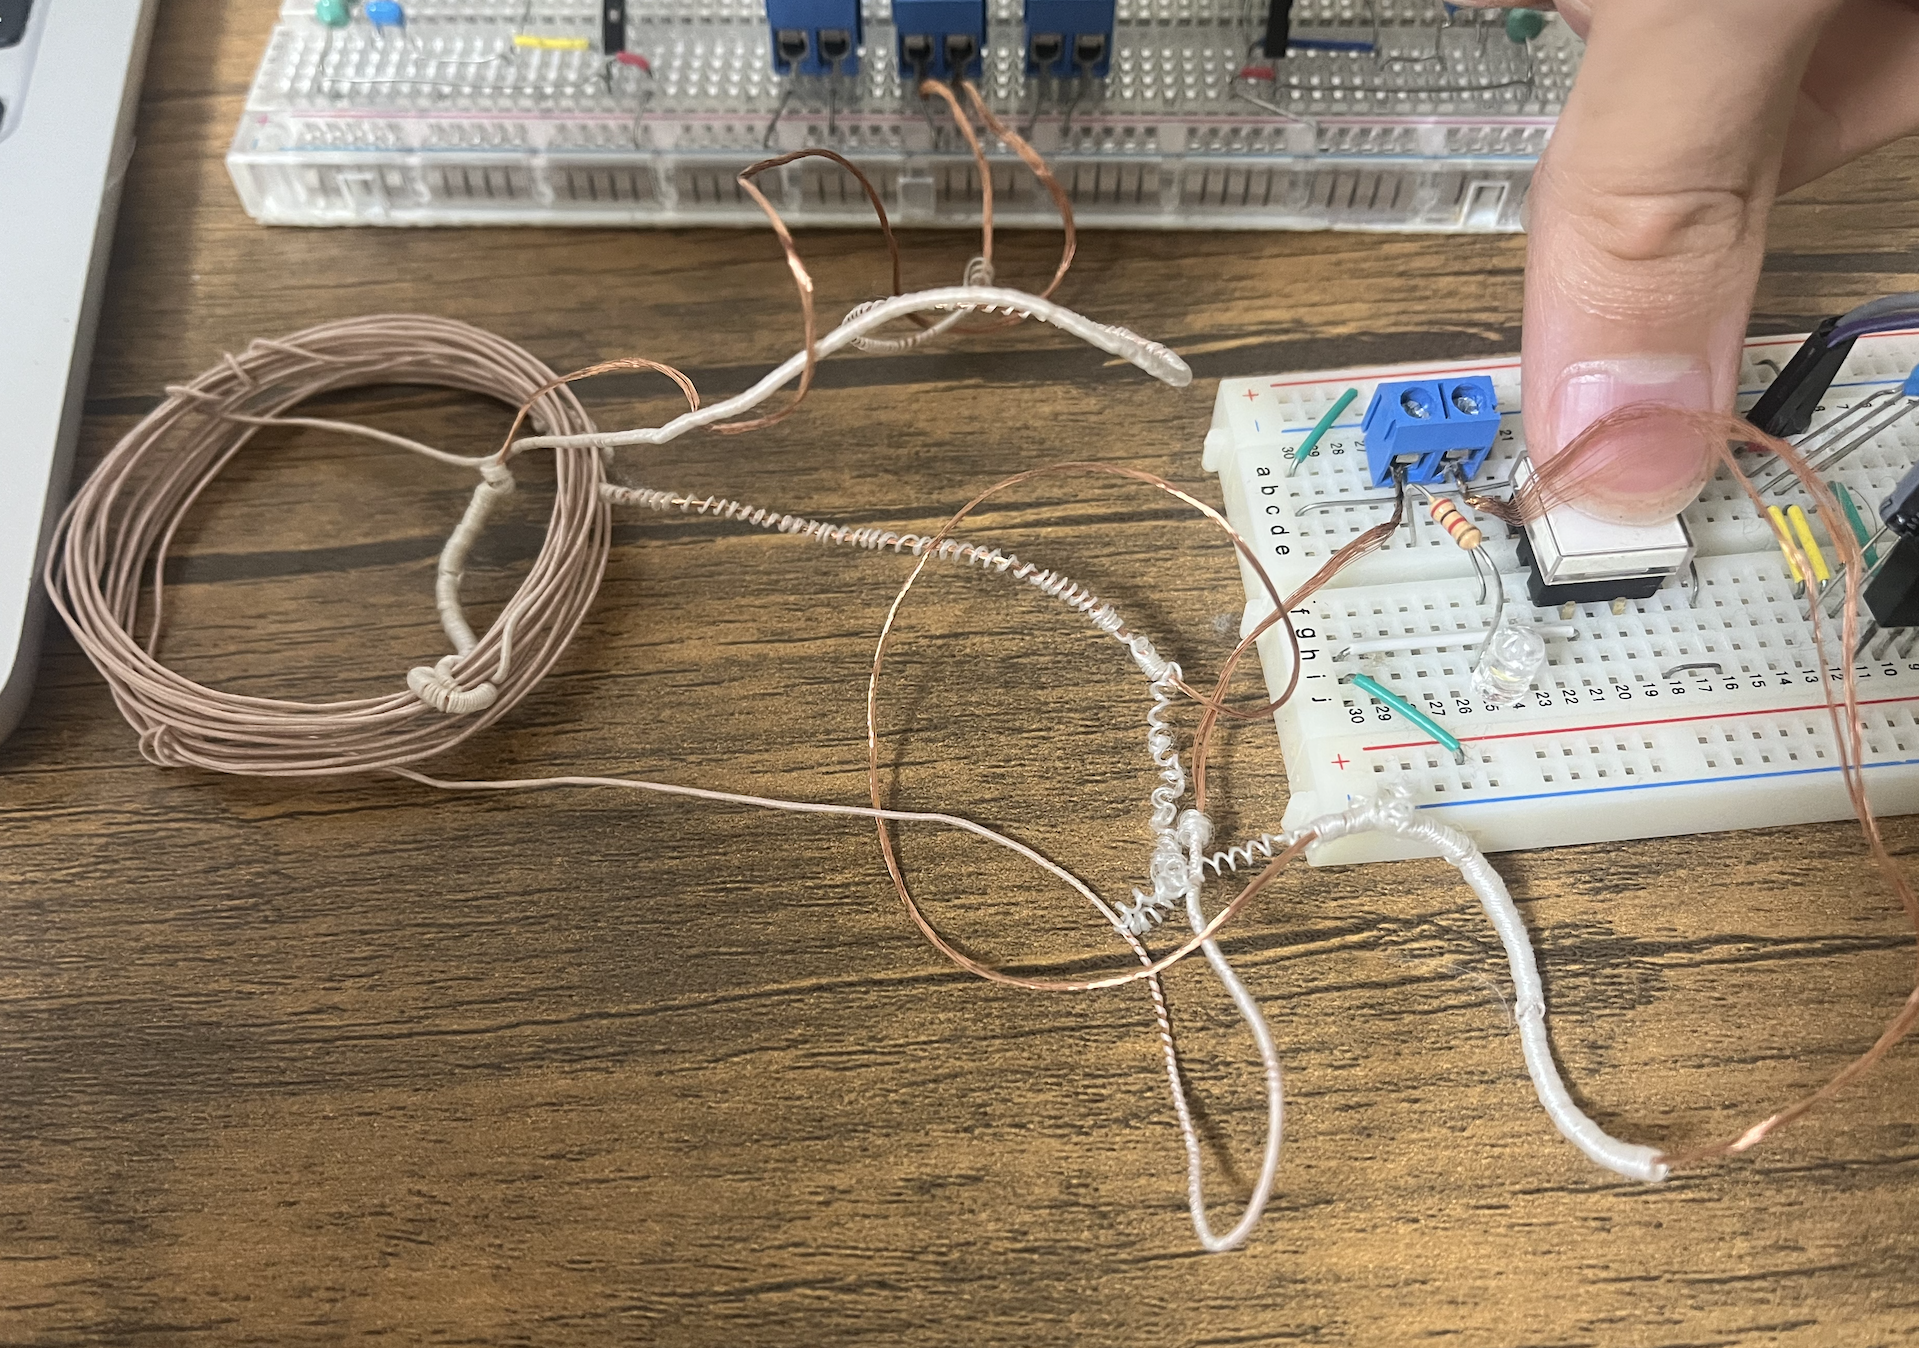
\includegraphics[width=0.8\linewidth]{./image/wireless5.png}
\caption{動作の様子。現在は受電側のコンデンサを外すことで電磁誘導方式として動作させるところまでできた。確かにコイルを近づけると白色LEDが光っていることがわかる。}
\end{figure}

したがって、これからはこの回路にコンデンサを追加して、個々の調整をうまくできるかどうかが開発のボトルネックになりそうである。この案について何かアドバイスがあったら、どんなことでもいいので教えていただきたい。よろしくお願いします。

\begin{thebibliography}{9}

\bibitem{taniguchi_bipolar}
バイポーラトラジスタ回路の設計,
\url{http://doku.bimyo.jp/bipoler/index.html}.

\bibitem{seo_lecture}
瀬尾 亨,
交通流のモデルとデータ (東京大学),
\url{https://bin.t.u-tokyo.ac.jp/model21/lecture/Seo.pdf}.

\bibitem{wiki_traffic_flow}
Wikipedia,
交通流理論,
\url{https://ja.wikipedia.org/wiki/交通流理論}.

\bibitem{wada_kwm_vt}
和田 健太郎:
交通流の Kinematic Wave モデルの解析法
Analysis Methods of Kinematic Wave Model of Traffic Flows,
\url{https://www.sk.tsukuba.ac.jp/~wadaken/PDF/JSTE/KWM-VT.pdf}.

\end{thebibliography}

\end{document}